\subsection{Implementasi Arsitektur \textit{Microservices} Menggunakan Komunikasi \textit{Event-Driven} Pada Aplikasi Pemesanan Tiket Acara (Jeeves)}

Tugas akhir ini membahas aplikasi pemesanan tiket acara dengan arsitektur \textit{microservice} dengan komunikasi \textit{event-driven}. Tujuan dari penelitian tersebut adalah membuat aplikasi tiket yang \textit{fault-tolerant} sehingga layanan yang masih berjalan tetap dapat memenuhi aksi yang lain. Untuk itu, arsitektur \textit{microservice} diimplementasikan dengan cara \textit{loosely-coupled}. Agar hal tersebut dapat dipenuhi, komunikasi \textit{event-driven} digunakan. Agar \textit{dependency} antarlayanan berkurang, seluruh data yang diperlukan oleh sebuah layanan diikutserkatan pada \textit{event} yang dikirim \parencite{microservicesEventDriven}.

\begin{figure}[ht]
    \centering
    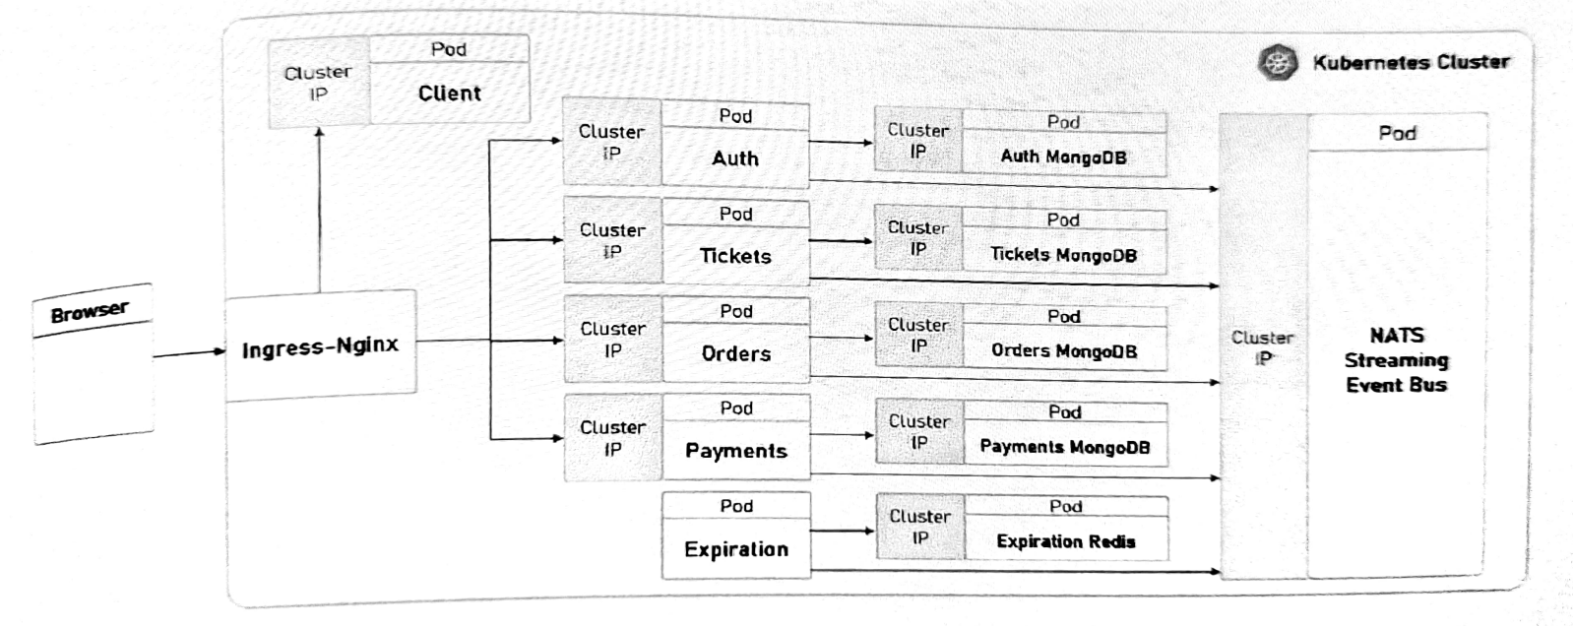
\includegraphics[width=1\textwidth]{resources/chapter-2/jeeves.png}
    \caption{Arsitektur Jeeves \parencite{microservicesEventDriven}}
    \label{fig:jeeves-architecture}
\end{figure}

Penelitian ini mengimplementasikan fungsionalitas dasar seperti otentikasi pengguna, pembuatan tiket, reservasi tiket, dan pembayaran tiket. Terdapat lima \textit{microservice} yang dibuat, yaitu layanan otentikasi, layanan tiket, layanan pemesanan, layanan pembayaran, dan \textit{expiration microservice}. Setiap layanaan selain \textit{expiration microservice} memiliki basis data masing-masing dengan menggunakan MongoDB. Hanya \textit{expiration microservice} yang menggunakan Redis. Selain itu, setiap komunikasi yang terjadi secara asinkron dilakukan melalui \textit{messaging platform} NATS. Untuk melakukan validasi otentikasi, sistem ini menggunakan JWT dengan \textit{shared secret} yang diatur oleh Kubernetes. Pendekatan ini memungkinkan layanan independen terhadap layanan otentikasi \parencite{microservicesEventDriven}.

Penelitian ini berhasil mengimplementasikan arsitektur aplikasi untuk pemesanan tiket acara yang \textit{fault-tolerant} dengan pendekatan \textit{microservice} dan \textit{event-driven}. Meskipun begitu, penelitian ini tidak membahas dan menguji aspek skalabilitas dan elastisitas dari sistem ini.